
\section{preliminaries}\label{sec:preliminaries}

\subsection{Lattices}\label{sec:lattices}
This section contains the definitions and theorems of lattices, complete lattices, and partial orders.
These definitions are necessary to understand the theory behind abstract interpretation.\cite{nielson_formal_2019}

\begin{definition}
    A \textit{partial order} $(S, \sqsubseteq)$ is set $S$ equipped with a binary relation $\sqsubseteq$ that is reflexive, transitive and anti-symmetric.
\end{definition}

For $X \sqsubseteq S$ and $y \in S$ we take
\begin{equation*}
    X \sqsubseteq y \iff \forall x \in X : x \sqsubseteq y,
\end{equation*}
and analogous for $y \sqsubseteq X$.

\begin{definition}
    A \textit{complete lattice} $(S, \sqsubseteq, \sqcup, \sqcap)$ is a partial order $(S, \sqsubseteq)$ in which for all $X \subseteq S:$ $\bigsqcup X$ and $\bigsqcap X$ are defined,
        \begin{equation*}
            X \sqsubseteq \bigsqcup X \land \forall y \in S : X \sqsubseteq y \implies \bigsqcup X \sqsubseteq y,
        \end{equation*}
        and
        \begin{equation*}
            \bigsqcap X \sqsubseteq X \land \forall y \in S : y \sqsubseteq X \implies y \sqsubseteq \bigsqcap X.
        \end{equation*}
\end{definition}

As a shorthand we take $x \sqcup y = \bigsqcup \{x, y\}$ and $x \sqcap y = \bigsqcap \{x, y\}$.

\begin{definition}
    A \textit{lattice} $(S, \sqsubseteq, \sqcup, \sqcap)$ is a partial order $(S, \sqsubseteq)$ in which for all $x,y \in S:$ $x \sqcup y$ and $x \sqcap y$ are defined,
        \begin{equation*}
            \{x, y\} \sqsubseteq x \sqcup y \land \forall z \in S : \{x, y\} \sqsubseteq z \implies x \sqcup y \sqsubseteq z,
        \end{equation*}
        and
        \begin{equation*}
            x \sqcap y \sqsubseteq \{x, y\} \land \forall z \in S : z \sqsubseteq \{x, y\} \implies z \sqsubseteq x \sqcap y.
        \end{equation*}
\end{definition}

\begin{theorem}\label{thm:kleene_finite}
    In a complete lattice $L$ with finite height, every monotone function $f : L \rightarrow L$ has a unique fixed point
    \begin{equation*}
        lfp(f) = \bigsqcup\{f^n(\perp) \mid n \in \mathbb{N}\}
    \end{equation*}.
\end{theorem}

\begin{theorem}\label{thm:kleene_scott}
    In a complete lattice $L$, every Scott-continuous function $f : L \rightarrow L$ has a unique fixed point $lfp(f)$.
\end{theorem}

\begin{theorem}
    If $L_1, L_2, \dots, L_n$ are complete lattices, the so is the product:
    \begin{equation*}
        L_1 \times L_2 \times \dots L_n = \{(x_1, x_2, \dots x_n) \mid x_i \in L_i\}
    \end{equation*}
    where the order $\sqsubseteq$ is defined componentwise:
    \begin{equation*}
        (x_1, x_2, \dots, x_n) \sqsubseteq (x_1', x_2', \dots, x_n')
        \iff
        \forall i = 1, 2, \dots n : x_i \sqsubseteq x_i'.
    \end{equation*}
\end{theorem}

\begin{theorem}
    If $A$ is a set and $L$ a complete lattice, then $L^A$ is a complete lattice when
    \begin{equation}
        f \sqsubseteq g \iff \forall a \in A : f(a) \sqsubseteq g(a) \text{ where } f,g \in L^A.
    \end{equation}

\end{theorem}

\todo[inline]{
    Casper says:
    The four theorems above should have a source.
}

\subsection{Abstract Interpretation}

\begin{theorem}\label{thm:galoispre}
    For $\gamma : L_1 \rightarrow L_2$ where $L_1$ and $L_2$ are complete lattices there exist a function $\alpha : L_2 \rightarrow L_1$ such that $\alpha$ and $\gamma$ forms a Galois connection if $\gamma(\bigsqcap B) = \bigsqcap_{b \in B}\gamma(b)$ for every $B \subseteq L_1$.
\end{theorem}

\subsection{Converting Code Program Graph}\label{subsection:converting-code-program-graph}
This section will briefly cover how the program graph is created.
Creating a program graph from the code is already a proven concept. Therefore, this paper will not delve into the details but inform the reader.
The book used to show that the concept of creating a program graph from code is a proven concept is~\cite[see][chap 2.2]{nielson_formal_2019}.
A program graph consists of a finite set of nodes, initial and final nodes, actions, and edges.

These directed edges represent the program's flow, and the nodes represent its state. The edges' actions are the atomic operations that the program can perform. The initial node is the program's starting point, and the final node is the program's end.

The program graph is created by parsing the code and creating nodes and edges that represent the flow of the code. This process, while it may sound complex, is actually quite straightforward. For instance, if the code is only an assignment of a variable, there will be a node for the initial state before the variable is assigned, a node for the final state after the variable is assigned, and an edge between them that represents the action of the assignment. This is written as the following equation:
$edges(q_{\circ} \rightsquigarrow q_{\bullet})\llbracket x:=a \rrbracket = \{(q_{\circ}, x:=a, q_{\bullet})\}$
$q_{\circ}$ is the initial node, $q_{\bullet}$ is the final node, and $x:=a$ is the assignment. This creates a set that represents the program graph, which can be seen in \autoref{fig:tikz-program-graph-assignment}. This is a simple example, and the program graph can be more complex depending on the code, but the concept is the same.
Further examples can be found in~\cite[Figure 2.6]{nielson_formal_2019}.

\begin{figure}[htb!]
    \center
    \begin{figure}[htb!]
    \center
    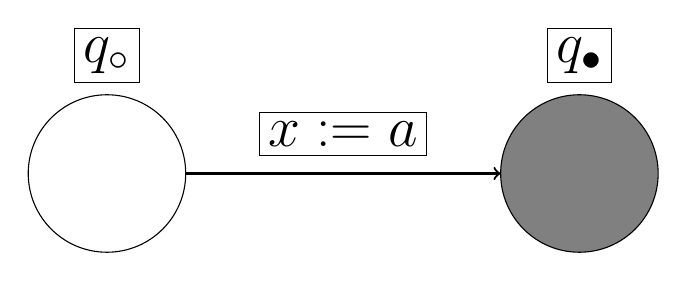
\begin{tikzpicture}
        \filldraw[fill=white, draw=black] (2,2) circle (1cm);
        \filldraw[fill=gray, draw=black] (8,2) circle (1cm);
        \node [draw] at (2,3.5) {\huge $q_{\circ}$};
        \node [draw] at (8,3.5) {\huge $q_{\bullet}$};
        \node [draw] at (5, 2.5) {\huge $x:=a$};
        \draw [thick, ->](3, 2) -- (7, 2);
    \end{tikzpicture}
    \caption{An example that shows a program graph of an assignment}
    \label{fig:tikz-program-graph-assignment}
\end{figure}
    \caption{An example that shows a program graph of an assignment}
    \label{fig:tikz-program-graph-assignment}
\end{figure}    